\documentclass{article}

\usepackage[english]{babel}
\usepackage[letterpaper,top=2cm,bottom=2cm,left=3cm,right=3cm,marginparwidth=1.75cm]{geometry}

\usepackage{amsmath}
\usepackage{graphicx}
\usepackage[colorlinks=true, allcolors=blue]{hyperref}
\usepackage{adjustbox}

\title{Homework 4 Report}
\author{Microl Chen}

\begin{document}
\maketitle

\section{Collaboration Statement}
For this assignment, the following resources, help, or/and collaboration was utilized:
\\Overleaf - for the Latex Template
\\Stack Overflow - minor error debugging
\\Debugged, diagnosed, and isolated errors with Programiz.com
\\Reference GeeksforGeeks for pageRank concepts
\\Graphviz tools was used to visualize graph


\section{Notes}
\subsection{Implementation Steps}
1. Cleaned the dot file by parsing the dot file as a string. \\
2. Created a makeshift abstract graph by making an artificial "edge list". \\
3. Created an adjacency matrix with the edge list. \\
4. Iterative-ly implemented pageRank using matrix multiplication at each step until it converges or reaches n (in my code I made it 100) times. \\
5. Sorted the pageRank scores.

\subsection{Dead Ends and Spider Traps}
Dead ends were dealt with by simply inputting a 0 in the adjacency matrix where the row and column represented the same node. This removed the possibility that values "get stuck" on a loop and allows for the standard page rank algorithm to reduce other dead end to 0. \\

\noindent
Spider Traps were dealt with by adding a teleportation probability. As discussed in class, by adding a dumping factor in our matrix multiplication, the program can get out of a loop that may be a potential spider trap.

\section{Results, Insights, and Other Experience}
My results were very expected (given that they were very simple graphs), when every edge had two directed edges in a cycle (reference figure 1 and 2), every node had the exact same page rank scores. When there was a dead end (variable because of teleportation), most of the time it has a lower page rank (figure 3). \\

From my test cases, I observed these following aspects in general:\\
1. Nodes with more edges generally score higher. \\
2. Nodes that are more accessible generally score higher. \\
3. Nodes in Spider Traps generally scored higher. \\

It is worth noting that many resources say that Spider Traps generally will score lower due to lower accessibility by a random surfer. I think my results differed slightly because of a lower sample size and more simplicity. \\

In terms of lessons learned, this assignment has really taught me alot more about numpy. There was so many numpy functions that existed that I was not aware of. In addition, Graphviz was a great tool to know of too, the application would have been great for note taking in CS253... Lastly, this assignment also taught me the power of approximation. Using the dumping factor method to soft force values to converge could be applied in so many different areas.

\section{TestCases}
\subsection{Figure 1: 5 Vertices, NO Dead End, No Spider}
Refer to the graph for the image. This is a simple graph that satisfies the requirement of not having any dead ends or spider traps. It is a directed cycle among five vertices.
\subsection{Figure 2: 10 Vertices, NO Dead End, No Spider}
Refer to the graph for the image. Similar to figure 1, this is a simple graph that satisfies the requirement of not having any dead ends or spider traps. It is a directed cycle among ten vertices.
\subsection{Figure 3: 10 Vertices, YES Dead End, No Spider}
Refer to the graph for the image. Graph 3 is simply figure 2, but with node J altered into a dead end.
\subsection{Figure 4: 10 Vertices, NO Dead End, YES Spider}
Refer to the graph for the image. Graph 4 has the same structure (for nodes A-G) as figures 1 and 2 - but with an added spider trap set that can be accessed by G. The set of nodes (H, I and J) is considered a spider trap because a traveler could not leave the set once they enter.
\subsection{Figure 5: 50 Vertices, NO Dead End, No Spider}
Refer to the graph for the image. Similar to figure 1 and 2, this is a simple graph that satisfies the requirement of not having any dead ends or spider traps. It is a directed cycle among 50 vertices with minor changes. Note that the graph is cut off because of its absurd length, and it did not make sense to portray the entire graph if it is simply a larger version of figure 1 and 2.

\begin{figure}
  \centering
  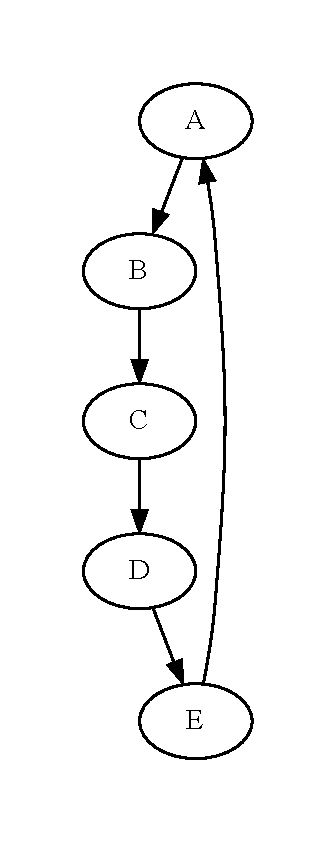
\includegraphics[width=0.5\textwidth]{graph1.pdf}
  \caption{5 Vertices, NO Dead End, No Spider}
  \label{fig:image_label}
\end{figure}

\begin{figure}
  \centering
  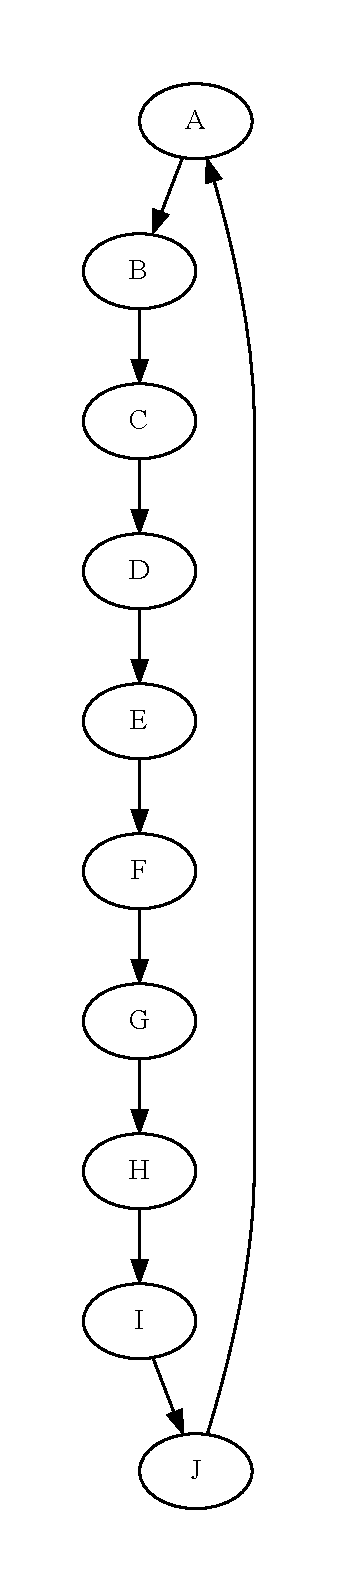
\includegraphics[width=0.32\textwidth]{graph2.pdf}
  \caption{10 Vertices, NO Dead End, No Spider}
  \label{fig:image_label}
\end{figure}
\begin{figure}
  \centering
  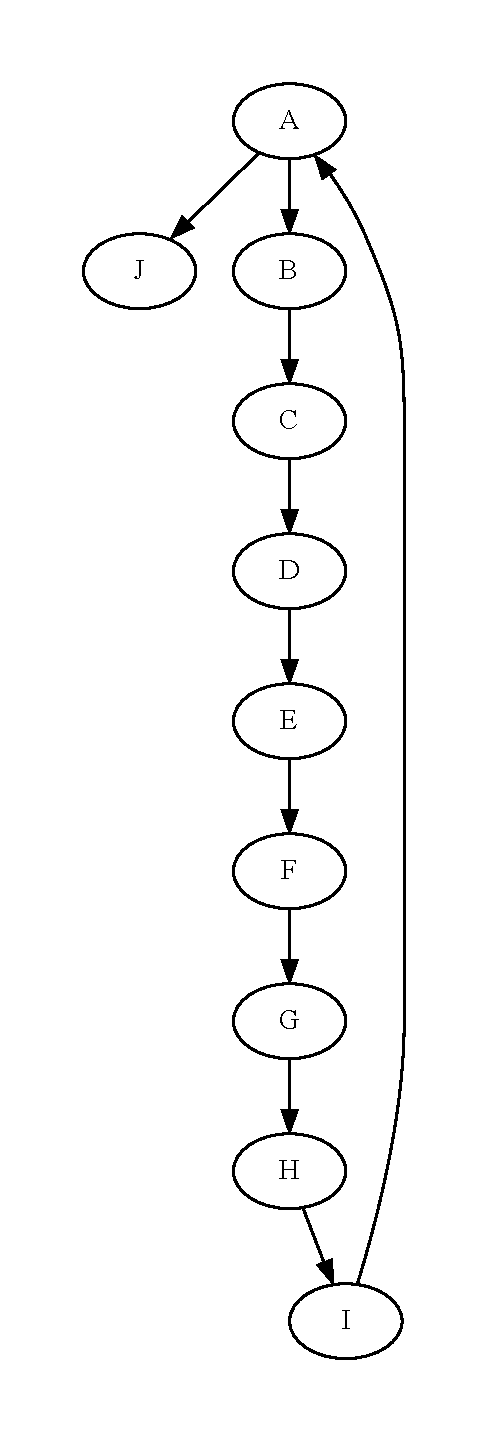
\includegraphics[width=0.5\textwidth]{graph3.pdf}
  \caption{10 Vertices, YES Dead End, No Spider}
  \label{fig:image_label}
\end{figure}
\begin{figure}
  \centering
  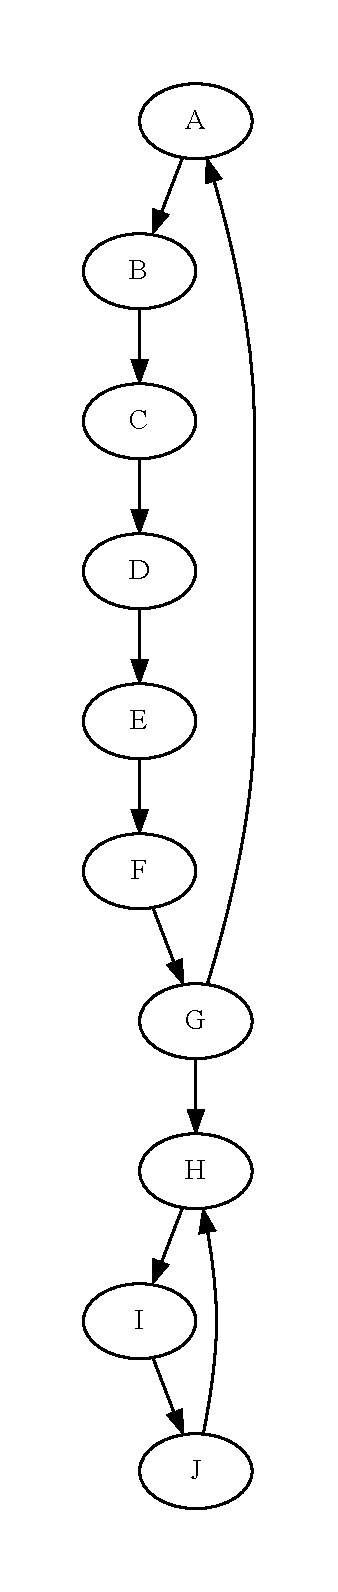
\includegraphics[width=0.32\textwidth]{graph4.pdf}
  \caption{10 Vertices, NO Dead End, YES Spider}
  \label{fig:image_label}
\end{figure}
\begin{figure}
  \centering
  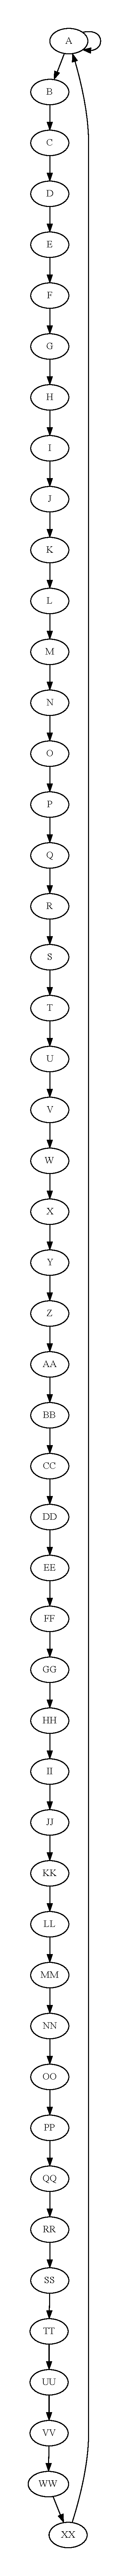
\includegraphics[width=0.4\textwidth]{graph5.pdf}
  \caption{50 Vertices, NO Dead End, No Spider}
  \label{fig:image_label}
\end{figure}
\end{document}